\section{Блок №2. Визуализация методов оптимизации и метод Ньютона}

\subsection{Постановка задачи}

\textbf{ДЗ2.1 (1 балл).} Написать программу для визуализации линий уровня целевой функции и ломаной последовательных приближений. Линии уровня должны проходить строго через вершины ломаной приближений (количество линий равно количеству приближений). Построить визуализацию для каждого метода оптимизации из ЛР4.

\textbf{ДЗ2.2 (1 балл).} Найти точку минимума функции численно методом Ньютона ($\varepsilon = 0.0001$). Выполнить решение также аналитически --- для каждой стационарной точки указать тип экстремума.

Данные по варианту:
\begin{equation}\label{eq:func2}
    z(x, y) = x^3 - 12x^2 + 45x + y^3 + 4y^2 + 4y - 54, \quad (x_0, y_0) = (4.5,\, -0.5).
\end{equation}

\subsection{Аналитическое решение (ДЗ2.2)}

Находим частные производные и приравниваем их к нулю:
\begin{align}
    \frac{\partial z}{\partial x} &= 3x^2 - 24x + 45 = 3(x - 3)(x - 5) = 0, \\
    \frac{\partial z}{\partial y} &= 3y^2 + 8y + 4 = (3y + 2)(y + 2) = 0.
\end{align}

Корни: $x \in \{3, 5\}$, $y \in \{-2/3, -2\}$. Получаем четыре стационарные точки.

Гессиан функции диагональный:
\begin{equation}
    H(x, y) = \begin{pmatrix}
        6x - 24 & 0 \\
        0 & 6y + 8
    \end{pmatrix}.
\end{equation}

Собственные значения: $\lambda_1 = 6x - 24$, $\lambda_2 = 6y + 8$.

\begin{table}[H]
    \centering
    \caption{Классификация стационарных точек}
    \label{tab:stationary}
    \begin{tabular}{|c|c|c|c|c|c|}
        \hline
        \textbf{Точка $(x, y)$} & \textbf{$\lambda_1$} & \textbf{$\lambda_2$} & \textbf{Тип} & \textbf{$z(x, y)$} \\
        \hline
        $(3, -0.6667)$ & $-6$ & $+4$ & Седловая точка & $-1.185185$ \\
        $(3, -2)$ & $-6$ & $-4$ & Локальный максимум & $0.000000$ \\
        $(5, -0.6667)$ & $+6$ & $+4$ & Локальный минимум & $-5.185185$ \\
        $(5, -2)$ & $+6$ & $-4$ & Седловая точка & $-4.000000$ \\
        \hline
    \end{tabular}
\end{table}

Глобальный минимум достигается в точке $(5, -2/3) \approx (5, -0.6667)$:
\begin{equation}
    z_{\min} = z\left(5, -\frac{2}{3}\right) = -5.185185.
\end{equation}

\subsection{Численное решение методом Ньютона (ДЗ2.2)}

Итерационная формула метода Ньютона:
\begin{equation}
    \mathbf{x}_{k+1} = \mathbf{x}_k - H^{-1}(\mathbf{x}_k) \nabla z(\mathbf{x}_k).
\end{equation}

Так как гессиан диагональный, обновления по $x$ и $y$ независимы:
\begin{equation}
    x_{k+1} = x_k - \frac{3x_k^2 - 24x_k + 45}{6x_k - 24}, \quad
    y_{k+1} = y_k - \frac{3y_k^2 + 8y_k + 4}{6y_k + 8}.
\end{equation}

Начальное приближение: $(4.5, -0.5)$, $\varepsilon = 0.0001$ (по норме градиента).

\begin{table}[H]
    \centering
    \caption{Итерации метода Ньютона}
    \label{tab:newton}
    \begin{tabular}{|c|c|c|c|c|}
        \hline
        \textbf{$k$} & \textbf{$x_k$} & \textbf{$y_k$} & \textbf{$z(x_k, y_k)$} & \textbf{$\|\nabla z\|$} \\
        \hline
        0 & 4.500000 & $-0.500000$ & $-4.500000$ & $2.37 \times 10^{0}$ \\
        1 & 5.250000 & $-0.650000$ & $-4.981500$ & $1.69 \times 10^{0}$ \\
        2 & 5.025000 & $-0.666463$ & $-5.183294$ & $1.52 \times 10^{-1}$ \\
        3 & 5.000305 & $-0.666667$ & $-5.185185$ & $1.83 \times 10^{-3}$ \\
        4 & 5.000000 & $-0.666667$ & $-5.185185$ & $2.79 \times 10^{-7}$ \\
        \hline
    \end{tabular}
\end{table}

Метод Ньютона сошёлся за 4 итерации. Численный результат $(5.000000, -0.666667)$ полностью совпадает с аналитическим $(5, -2/3)$.

Характерна квадратичная сходимость: на каждой итерации норма градиента уменьшается примерно на порядок (от $10^{0}$ до $10^{-1}$, затем до $10^{-3}$, затем до $10^{-7}$).

\subsection{Методы оптимизации и визуализация (ДЗ2.1)}

Реализованы четыре метода оптимизации:

\begin{enumerate}
    \item \textbf{Градиентный спуск} с постоянным шагом ($\alpha = 0.05$):
    \begin{equation}
        \mathbf{x}_{k+1} = \mathbf{x}_k - \alpha \nabla z(\mathbf{x}_k).
    \end{equation}

    \item \textbf{Наискорейший спуск} с одномерным поиском методом золотого сечения:
    \begin{equation}
        \mathbf{x}_{k+1} = \mathbf{x}_k - \alpha_k \nabla z(\mathbf{x}_k), \quad
        \alpha_k = \arg\min_{\alpha > 0} z(\mathbf{x}_k - \alpha \nabla z(\mathbf{x}_k)).
    \end{equation}

    \item \textbf{Метод сопряжённых градиентов} (формула Флетчера--Ривса):
    \begin{align}
        \mathbf{d}_0 &= -\nabla z(\mathbf{x}_0), \\
        \beta_k &= \frac{\|\nabla z(\mathbf{x}_{k+1})\|^2}{\|\nabla z(\mathbf{x}_k)\|^2}, \\
        \mathbf{d}_{k+1} &= -\nabla z(\mathbf{x}_{k+1}) + \beta_k \mathbf{d}_k.
    \end{align}

    \item \textbf{Метод Ньютона} (см. раздел~\ref{tab:newton}).
\end{enumerate}

\begin{table}[H]
    \centering
    \caption{Результаты методов оптимизации из начальной точки $(4.5, -0.5)$}
    \label{tab:methods}
    \begin{tabular}{|l|c|c|c|}
        \hline
        \textbf{Метод} & \textbf{Итераций} & \textbf{Финальная точка} & \textbf{$z_{\min}$} \\
        \hline
        Градиентный спуск ($\alpha = 0.05$) & 39 & $(4.999999, -0.666643)$ & $-5.185185$ \\
        Наискорейший спуск & 1 & $(5.000000, -0.666667)$ & $-5.185185$ \\
        Сопряжённые градиенты & 1 & $(5.000000, -0.666667)$ & $-5.185185$ \\
        Метод Ньютона & 4 & $(5.000000, -0.666667)$ & $-5.185185$ \\
        \hline
    \end{tabular}
\end{table}

\textbf{Замечание.} Наискорейший спуск и метод сопряжённых градиентов сошлись за 1 итерацию, так как функция сепарабельна (нет перекрёстных членов $xy$), а градиент в начальной точке $(4.5, -0.5)$ направлен точно в минимум $(5, -2/3)$:
\begin{equation}
    -\nabla z(4.5, -0.5) = (2.25, -0.75), \quad
    \frac{5 - 4.5}{2.25} = \frac{-2/3 - (-0.5)}{-0.75} = \frac{2}{9} \approx 0.2222.
\end{equation}

На рисунке~\ref{fig:all_methods} показаны линии уровня целевой функции и ломаная последовательных приближений для четырёх методов. Линии уровня проходят через вершины ломаной: число линий равно числу приближений (ключевое требование ДЗ2.1).

\begin{figure}[H]
    \centering
    \begin{subfigure}{0.48\textwidth}
        \centering
        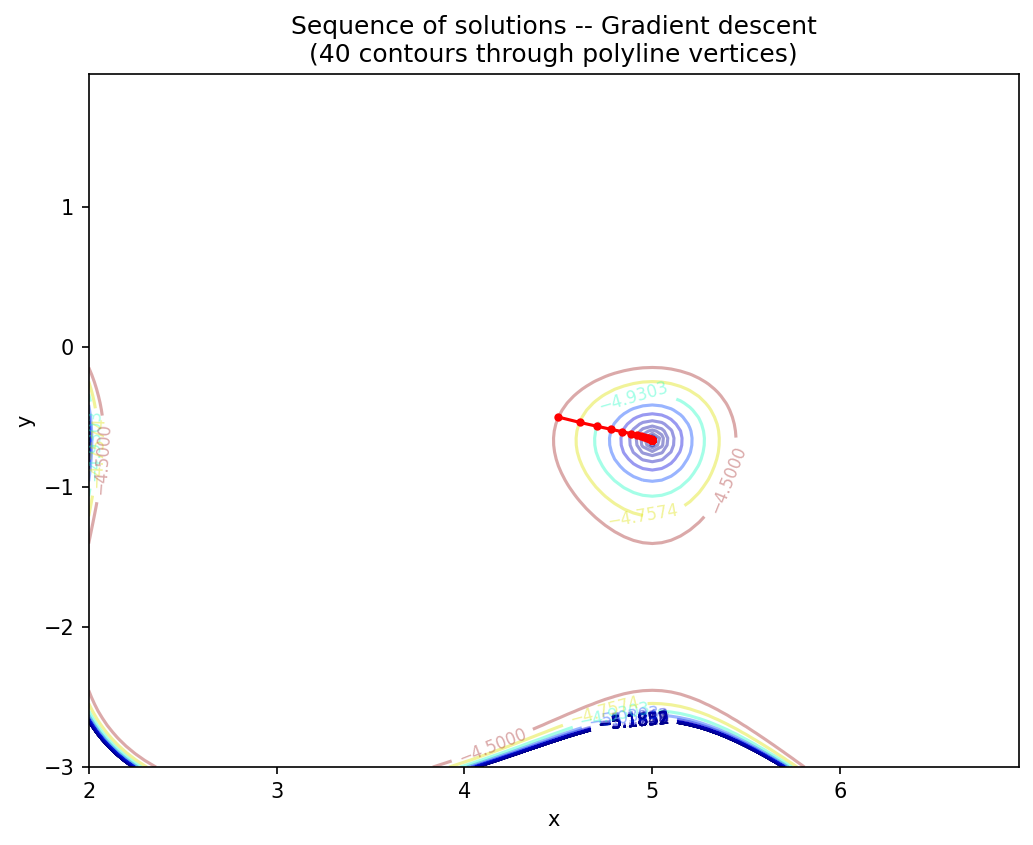
\includegraphics[width=\textwidth]{pic/level_lines_gradient_descent.png}
        \caption{Градиентный спуск ($\alpha = 0.05$): 39 итераций}
        \label{fig:gd}
    \end{subfigure}
    \hfill
    \begin{subfigure}{0.48\textwidth}
        \centering
        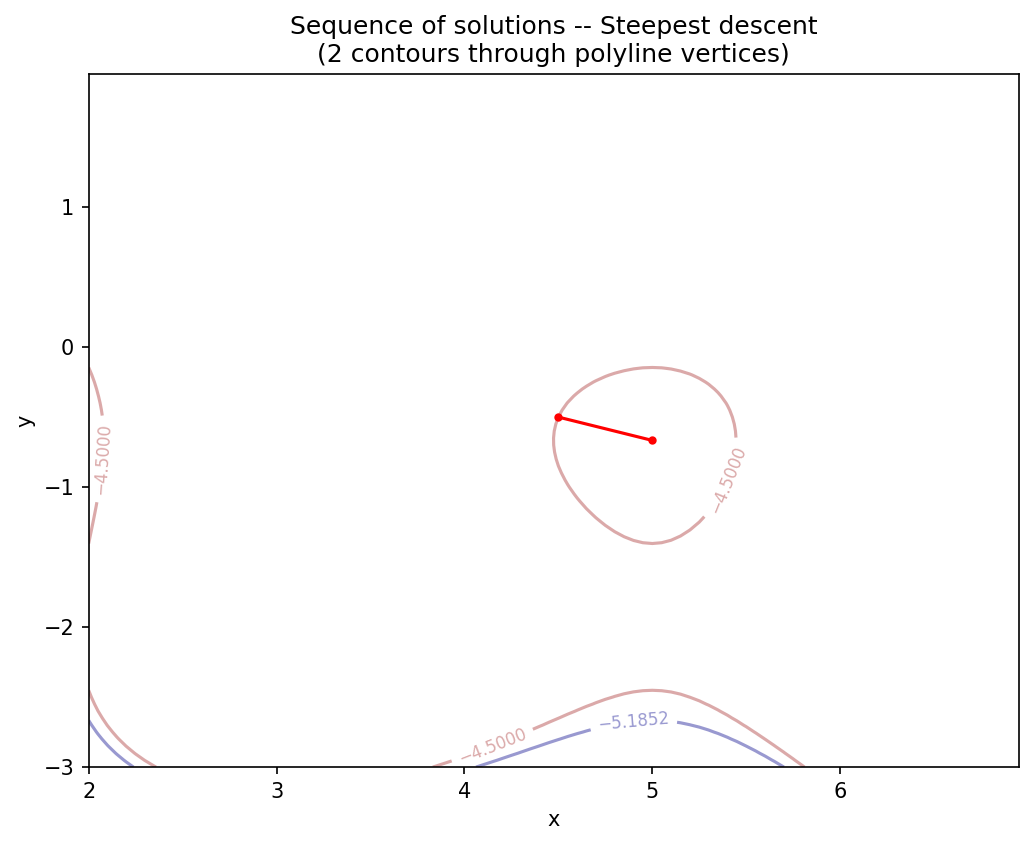
\includegraphics[width=\textwidth]{pic/level_lines_steepest_descent.png}
        \caption{Наискорейший спуск: 1 итерация}
        \label{fig:sd}
    \end{subfigure}

    \vspace{\baselineskip}

    \begin{subfigure}{0.48\textwidth}
        \centering
        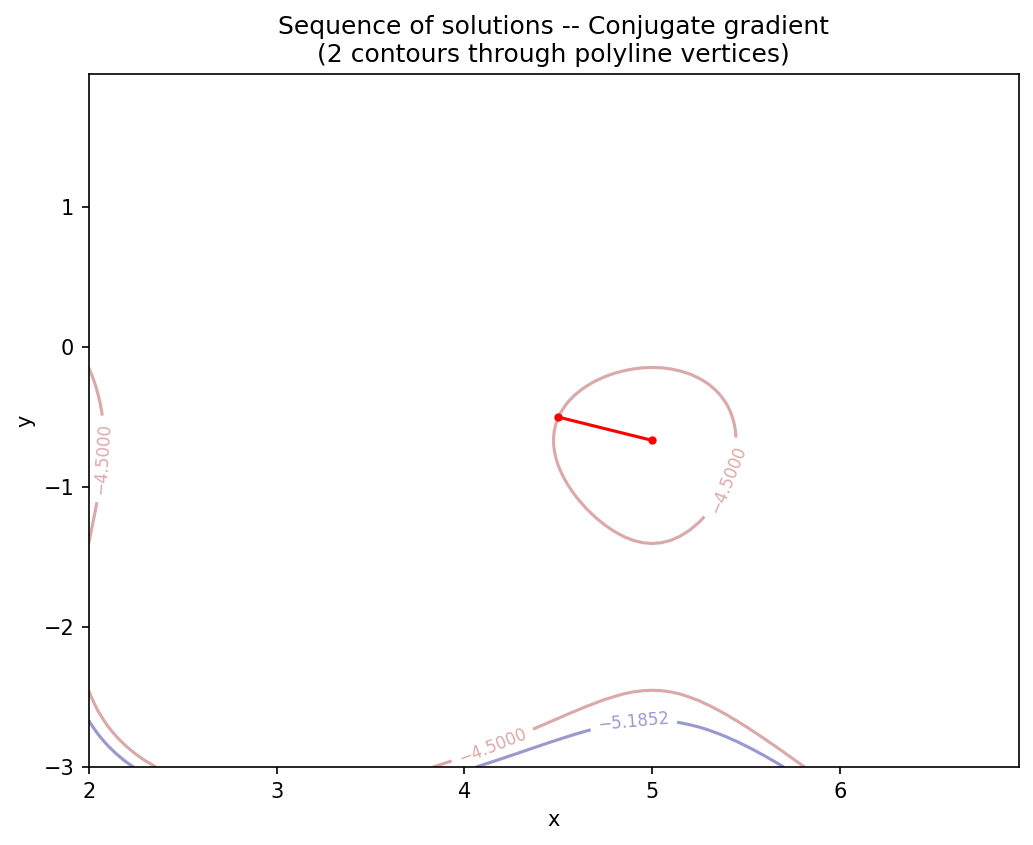
\includegraphics[width=\textwidth]{pic/level_lines_conjugate_gradient.png}
        \caption{Метод сопряжённых градиентов: 1 итерация}
        \label{fig:cg}
    \end{subfigure}
    \hfill
    \begin{subfigure}{0.48\textwidth}
        \centering
        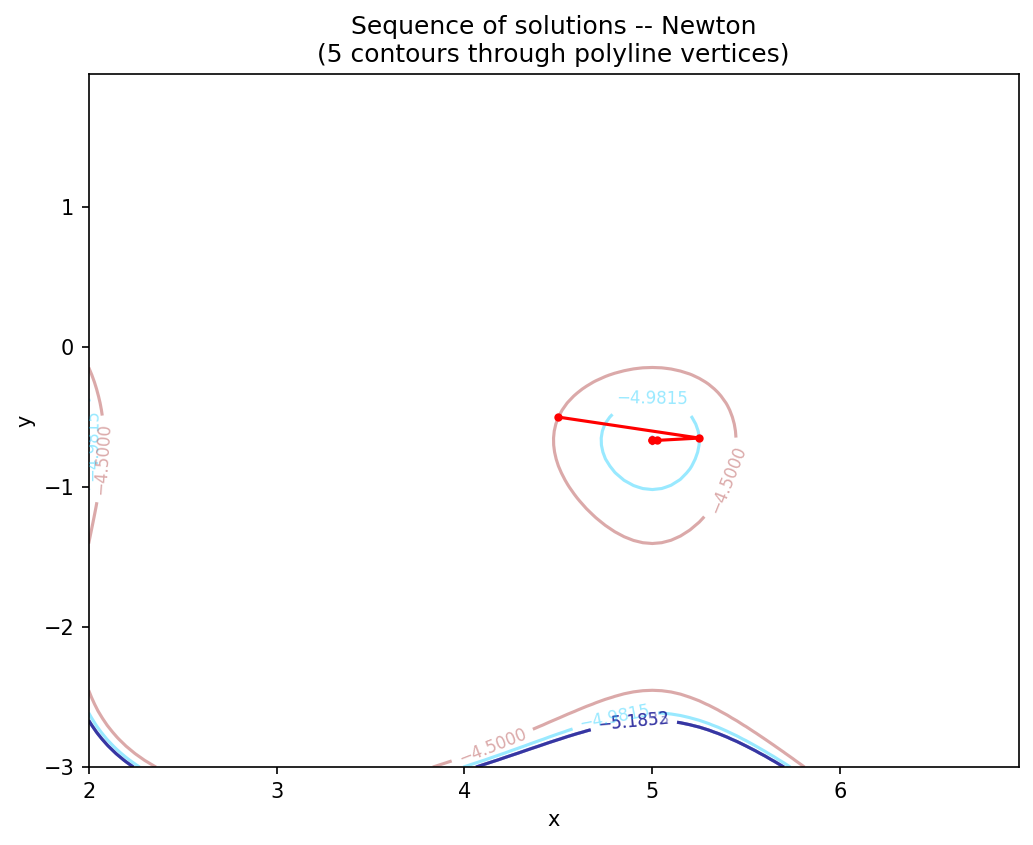
\includegraphics[width=\textwidth]{pic/level_lines_Newton.png}
        \caption{Метод Ньютона: 4 итерации}
        \label{fig:newton}
    \end{subfigure}
    \caption{ДЗ2.1: Визуализация четырёх методов оптимизации. Линии уровня проходят через вершины ломаной приближений.}
    \label{fig:all_methods}
\end{figure}

\subsection{Вывод}

Аналитическое исследование выявило четыре стационарные точки, из которых одна является глобальным минимумом $(5, -2/3)$. Численное решение методом Ньютона сошлось к этому минимуму за 4 итерации с квадратичной скоростью.

Все четыре метода оптимизации успешно находят минимум. Наискорейший спуск и сопряжённые градиенты демонстрируют исключительно быструю сходимость (1 итерация) благодаря удачному направлению градиента из начальной точки. Градиентный спуск с постоянным шагом сходится медленнее (39 итераций), но гарантированно. Метод Ньютона обеспечивает наилучший баланс скорости и точности.

Визуализация подтверждает, что линии уровня проходят строго через вершины ломаной приближений для каждого метода.
